Zur Erstellung der Android-App wurde AppInventor(\url{https://appinventor.mit.edu/}) und 
die BLE-Extension verwendet.\\
Geschrieben wurde das Programm von mir. Ideen und Anregungen wurden in verschiedensten 
Foren gefunden. \\
\\
Beim Start der App wird man aufgefordert Bluetooth und GPS anzuschalten, das GPS
ist nach Android-Richtlinien zu aktivieren. Danach kann man nach verschiedenen
Geräten scannen und sich mit diesen zu verbinden. Erfolgt die Verbindung mit einem
falschen Gerät schließt sich die App.\\
Nach der Verbindung wird sofort die Übertragung gestartet\\
\\
Das empfangene Datenpaket muss vor der Verarbeitung in die einzelnen Daten
aufgespalten und von String zu mindestens Float-Werten gepaarst werden.
Die Split-Funktion von AppInventor sucht nach `` $|$ '' als Trennzeichen und spaltet
hier die Werte. Diese werden in ein Array gespeichert welches später
die einzelnen aktuellen Werte ausgeben kann.\\
Es gibt insgesamt 3 Möglichkeiten die Daten anzeigen zu lassen.

\subsection{Rohdaten}
Die gelesenen Daten werden direkt im Textformat auf dem Bildschirm ausgegeben.
Der Zeitunterschied zwischen Datenpaketen wird in Millisekunden auf dem Bildschirm
angezeigt.
Es ist möglich die Daten gleichzeitig aufzuzeichnen.

\subsection{Graph}
Die Beschleunigungs-Daten werden in einem Graph dargestellt, hierzu werden sie zuerst in ein
Array geschrieben. Aus diesem Array erzeugt das Programm in einem vorgegebene Bereich
die Datenpunkte, die aufgrund ihrer Masse wie ein Liniendiagramm aussehen.\\
Neue Daten werden rechts geschrieben, während die alten Daten nach Links aus dem
Bildschirm verschwinden.\\
Der Zeitunterschied zwischen Datenpaketen wird in Millisekunden auf dem Bildschirm
angezeigt.
Es ist möglich die Daten gleichzeitig aufzuzeichnen.\\

\begin{figure} [h]
    \centering
    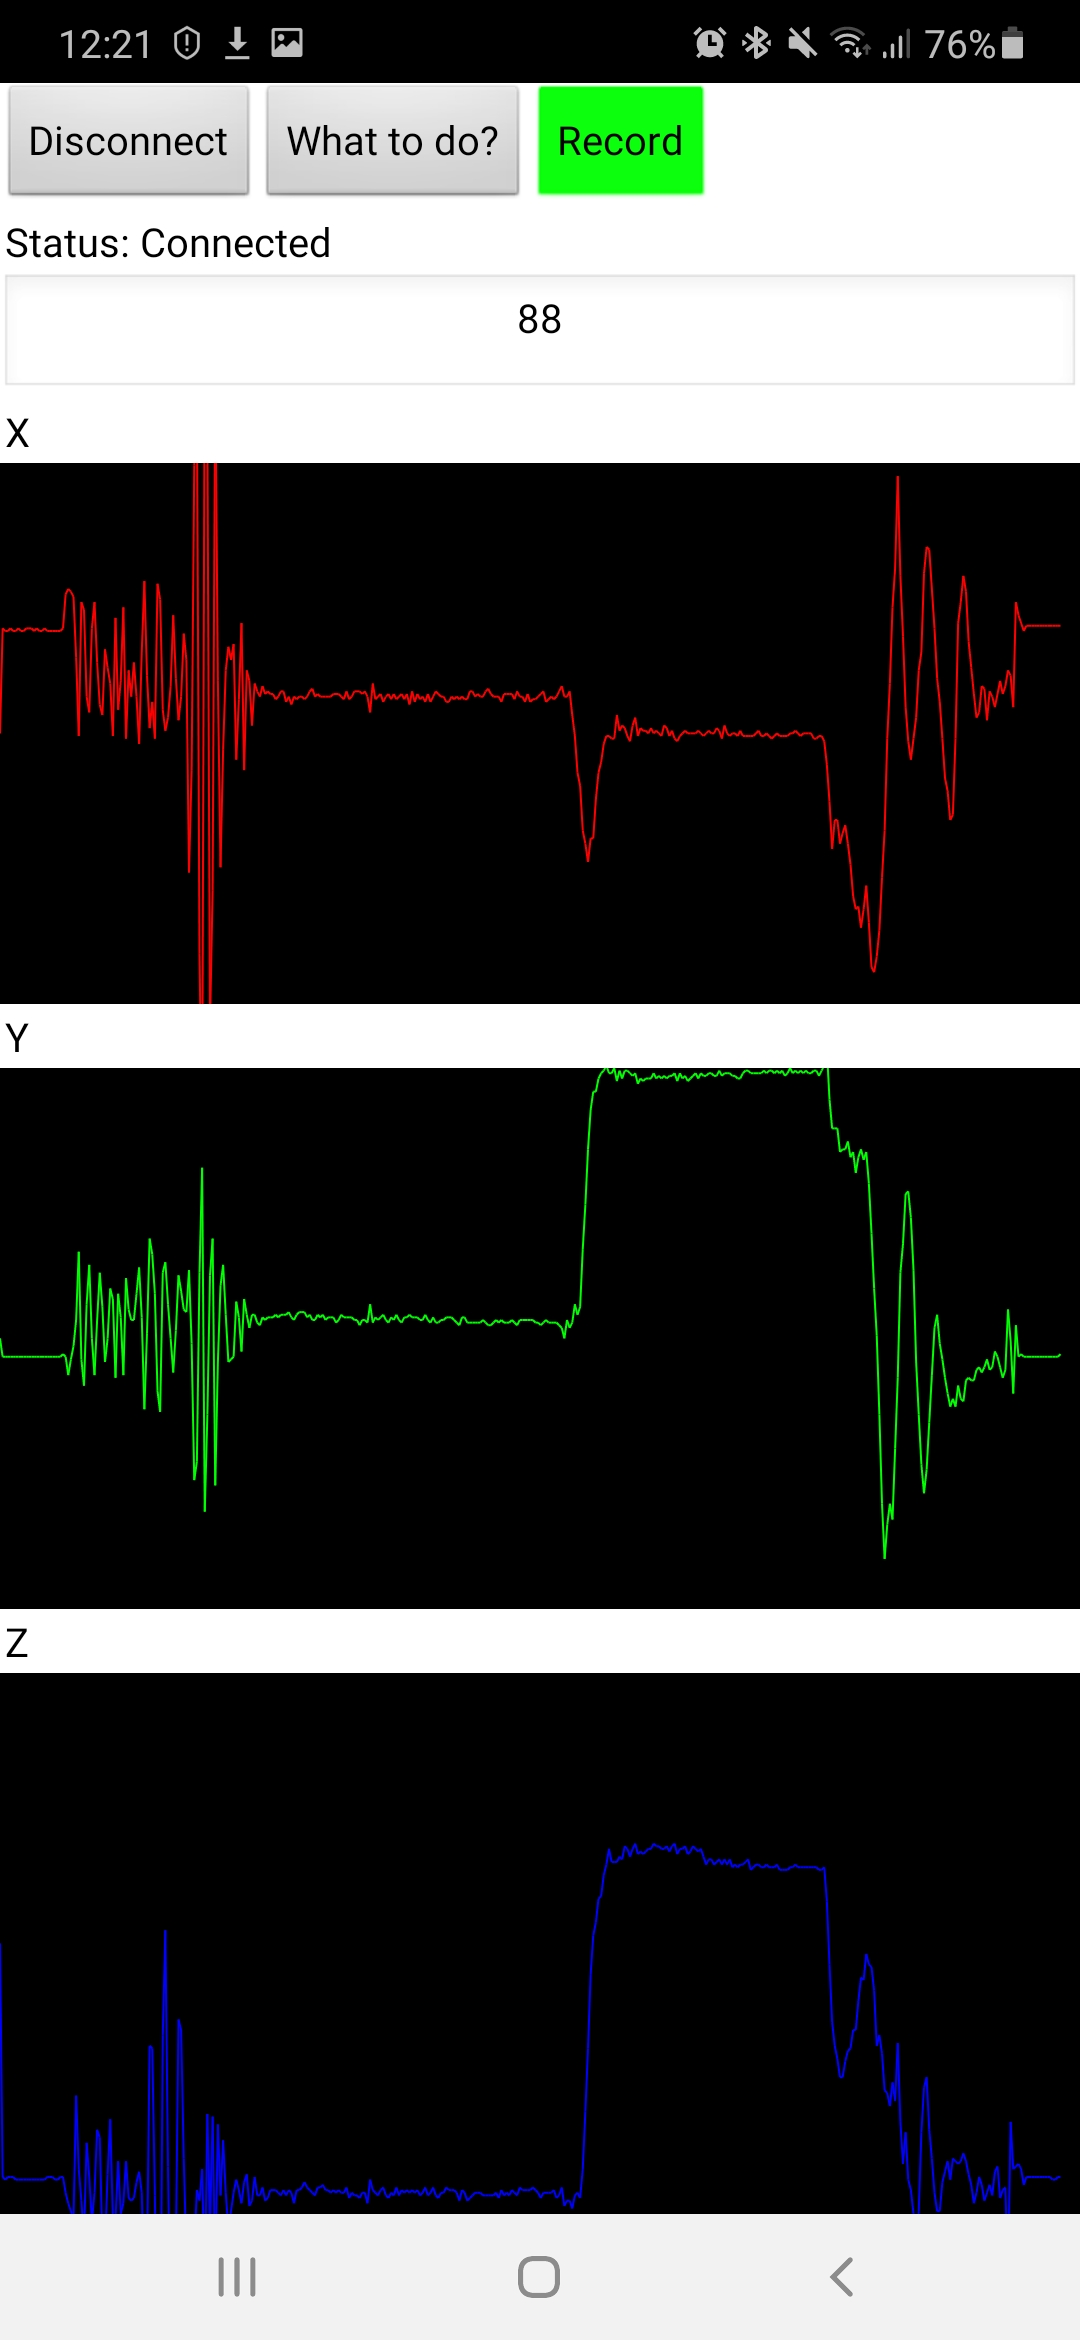
\includegraphics[height = 7cm]{Bilder/Graph}
    \caption{Live-Graph}
    %\label{fig:wo-bin-ich}
    \end{figure}

\subsection{Animation}
Hier wird die Distanz aus den Beschleunigungsdaten berechnet und mithilfe eines Punktes
visualisiert. Benutzt werden hierfür die X- und Y-Achse. Die Rechnung kann man in 
\refname { 5.4.1 Gleichmäßige Formel} einsehen.
%das Wort Kapitel steht da blöd....
\subsection{Aufgezeichnete Daten}
Die von den anderen Funktionen aufgezeichneten Funktionen können hier ausgegeben
werden. Hierzu benötigt der Schütze den Namen der Datei. Die Dateien werden
seit kurzem unter Android in einem App-Eigenem Ordner gespeichert. Diesen muss
der Schütze momentan auslesen um den zufälligen Namen der neuen Datei zu kennen.\\
Die Daten werden als Graph dargestellt. Die Beschleunigungsdaten werden außerdem
in Rohform über dem Graphen ausgegeben.\\

\begin{figure} [h]
    \centering
    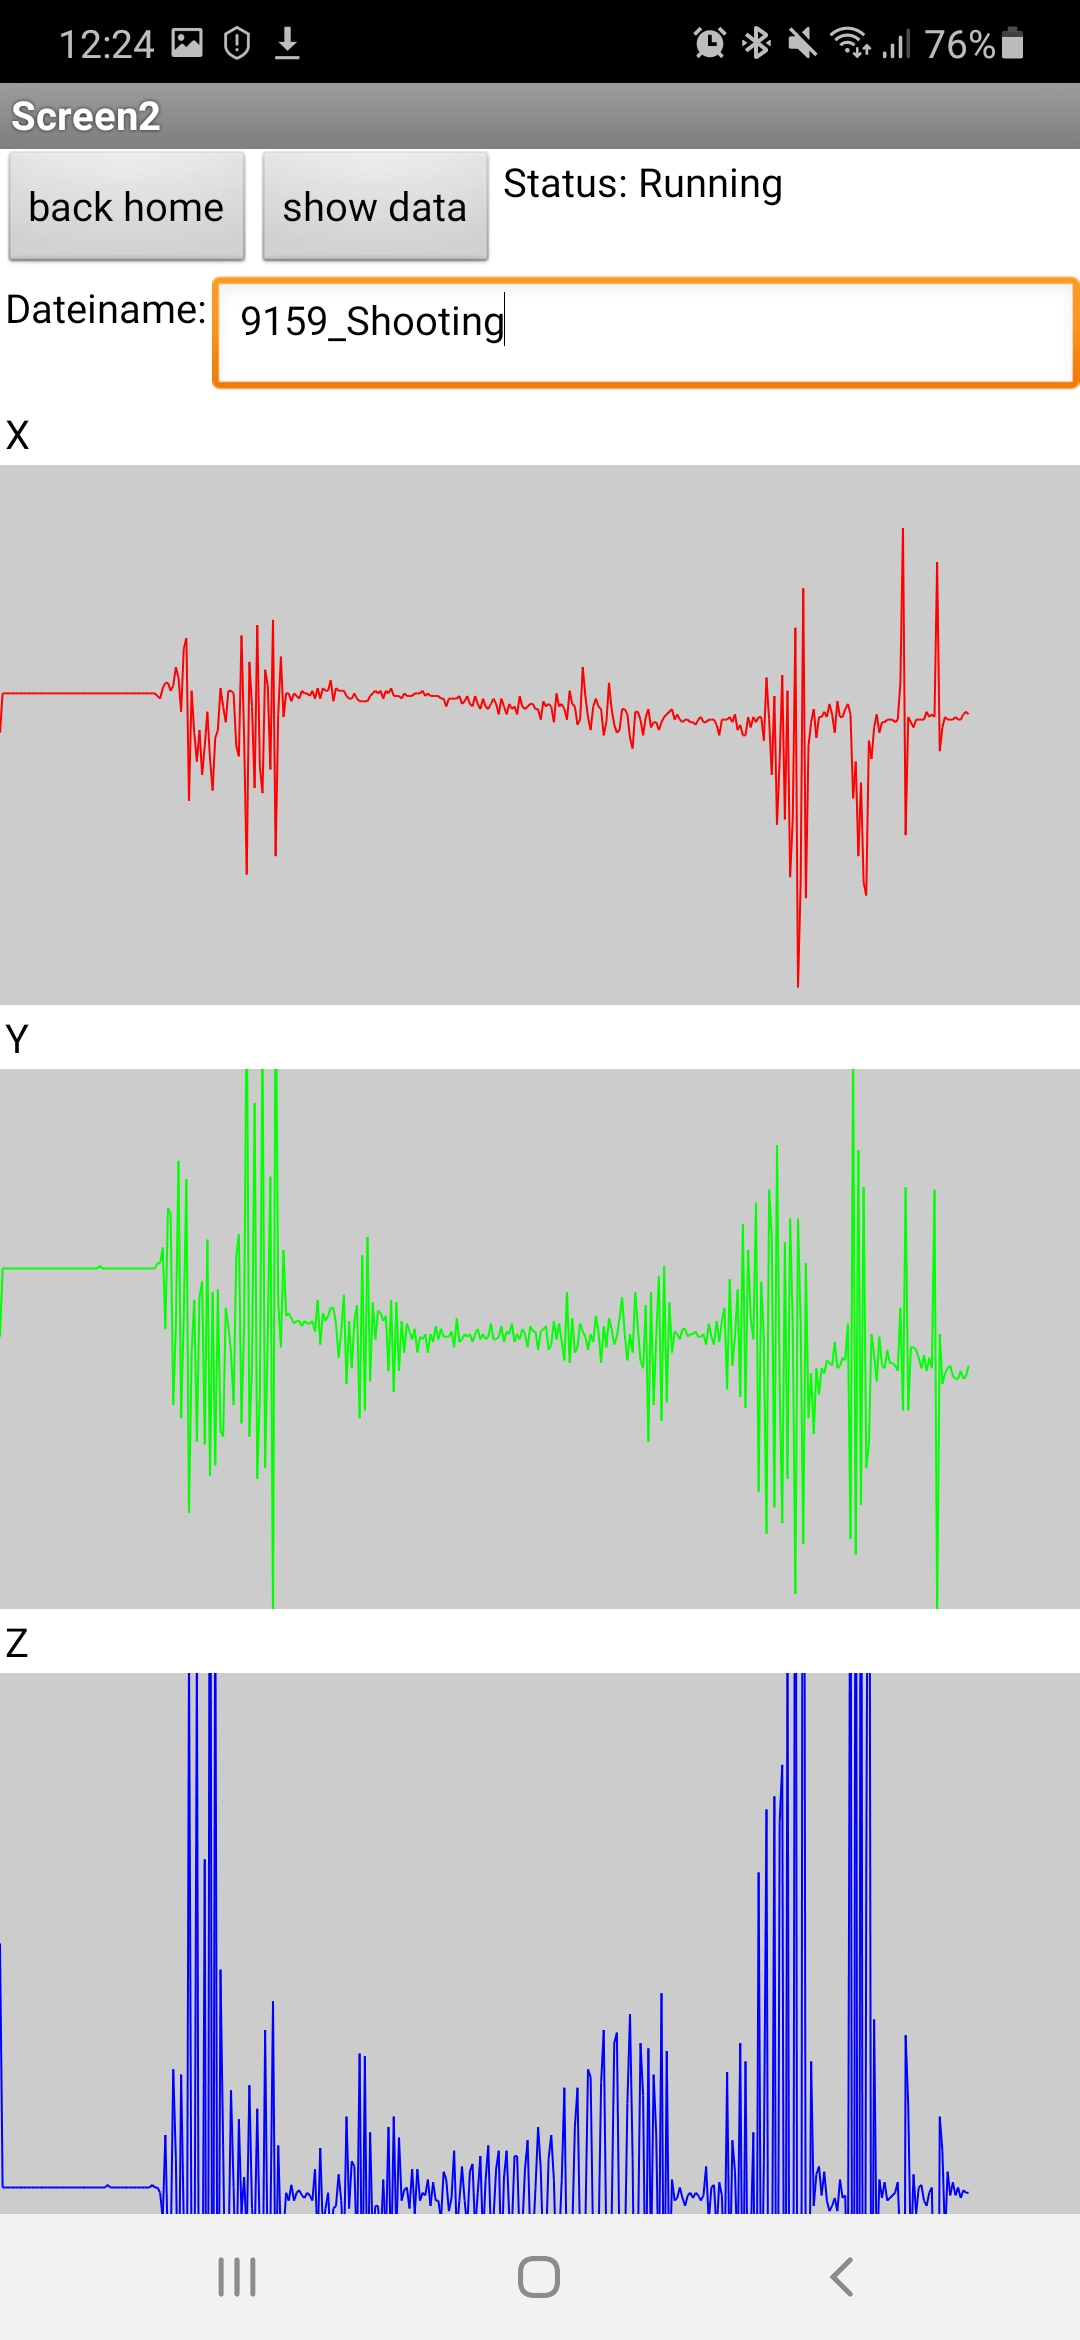
\includegraphics[height = 7cm]{Bilder/GraphRec}
    \caption{Aufgezeichneter Graph}
    %\label{fig:wo-bin-ich}
    \end{figure}


%Wie lasse ich den Text um das Bild fließen?